\documentclass[a4paper,14pt]{article}

\input{lab_Preamble.tex}


\begin{document}
\author{Рябых Владислав и Исыпов Илья, Б05-905}
\title{\tbf{Лабораторная работа № 3.2.4 \\ Свободные колебания в электрическом контуре}}
\maketitle

\tbf{Цель работы:} исследование свободных колебаний в электрическом колебательном контуре.

\tbf{В работе используются:} генератор импульсов, электронное реле, магазин сопротивлений, магазин ёмкостей, индуктивность, электронный осциллограф с разделительной панелью, измеритель $LCR$.


\section*{Теория}


\begin{center}
	\begin{figure}[bhtp]
		\centering
		\includegraphics[width=0.35\linewidth]{RLC.png}
		\caption{Колебательный контур}
		\label{RLC}
	\end{figure}
\end{center}

Основное уравнение колебательного контура 

\begin{equation}\label{ddot I}
\ddot{I} + 2\gamma\dot{I} + \omega_0^2I = 0
\end{equation}

Где $ \gamma = \dfrac{R}{2L} $ --- коэффициент затухания, $ \omega_0^2 = \dfrac{1}{LC} $ --- собственная частота контура. Решением этого уравнения являются затухающие колебания:

\begin{equation*}\label{}
I = A e^{-\gamma t} \cos (\omega t - \theta)
\end{equation*}

Здесь $ \omega = \sqrt{\omega_0^2 - \gamma^2} $. Можно записать решение \eqref{ddot I} и для напряжения:

\begin{equation*}\label{}
U_C = U_0 \dfrac{\omega_0}{\omega} e^{-\gamma t}\cos (\omega t - \theta)
\end{equation*}

В контуре со слабым затуханием $ (\omega \backsimeq \omega_0) $ верна \textbf{формула Томпсона} для периода: 

\begin{equation*}\label{}
T = \dfrac{2\pi}{\omega_0} \backsimeq  \dfrac{2\pi}{\omega} = 2\pi\sqrt{LC}
\end{equation*}

Режим работы контура, при котором $ \gamma = \omega_0 $, называется \textbf{критическим}. Его сопротивление равно 

\begin{equation}\label{Rkr}
R_\text{кр} = 2\sqrt{\dfrac{L}{C}}
\end{equation}

Потери затухающих колебаний принято характеризовать через \textbf{добротность} и \textbf{логарифмический декремент затухания}: 

\begin{equation}\label{Q}
Q = 2\pi \dfrac{W}{\Delta W} = \dfrac{1}{R} \sqrt{\dfrac{L}{C}} \quad - \quad \text{Добротность, потери энергии}
\end{equation}
\begin{equation}\label{theta}
\Theta = \dfrac{1}{n} \gamma T = \dfrac{1}{n} \ln \dfrac{U_k}{U_{k+n}}  \quad - \quad \text{Лог. декремент, потери амплитуды}
\end{equation}



\section*{Экспериментальная установка}
На рис. \ref{scheme} приведена схема для исследования
свободных колебаний в контуре, содержащем постоянную индуктивность $L$ и переменные ёмкость $C$ и сопротивление $R$. Колебания наблюдаются на экране осциллографа.
Для периодического возбуждения колебаний в контуре используется генератор
импульсов Г5-54. С выхода генератора по коаксиальному кабелю импульсы поступают на колебательный контур через электронное реле, смонтированное в отдельном блоке (или на выходе генератора). Реле содержит диодный тиристор $D$
и ограничительный резистор $R_1$.


\begin{center}
	\begin{figure}[bhtp]
		\centering
		\includegraphics[width=0.7\linewidth]{scheme.png}
		\caption{Схема установки для исследования свободных колебаний}
		\label{scheme}
	\end{figure}
\end{center}


Импульсы заряжают конденсатор $C$. После каждого импульса генератор отключается от колебательного контура, и в контуре возникают свободные затухающие колебания. Входное сопротивление осциллографа велико ($\simeq$ 1 МОм), так что
его влиянием на контур можно пренебречь. Для получения устойчивой картины
затухающих колебаний используется режим ждущей развёртки с синхронизацией
внешними импульсами, поступающими с выхода <синхроимпульсы> генератора.

\section*{Ход работы}

\subsection*{Измерение периодов}

Проведем измерения при $ R = 0 $. Будем изменять ёмкость от 0.02 до 0.90 мкФ, проводя измерения периода по формуле $T_{\text{эксп}} = T_0 \dfrac{x}{nx_0}$,
где $ T_0 = 0.01 $ c, $ x_0 $ --- расстояние одного импульса, $ x $ --- расстояние $ n $ импульсов. Погрешность $ \sigma_x = \sigma_{x_0} = 0.1, \sigma_{T_0} = 0.001  $c, тогда 
$$\sigma_{T_{\text{эксп}}} = T_{\text{эксп}} \sqrt{ \left( \dfrac{ \sigma_x}{x} \right)^2 + \left( \dfrac{ \sigma_{x_0}}{x_0} \right)^2  +  \left( \dfrac{ \sigma_{T_0}}{T_0} \right)^2}$$
а $ T_{\text{теор}} = 2\pi\sqrt{LC} $, где $ L = 136 $ мГн, $ \sigma_L = 5 $ мГн. $ \dfrac{\sigma_C}{C} \approx 0 $. Тогда $\sigma_{T_{\text{теор}}} = T_{\text{теор}} \cdot \dfrac{1}{2} \dfrac{\sigma_L}{L}$

Результаты измерений приведены в таблице \ref{tab1}.

\begin{table}[hbt!]
	\begin{center}
	\begin{tabular}{|c|c|c|c|c|c|}
		\hline
		$C$, мкФ & $n$  & $T_{\text{эксп}}$, мc & $T_{\text{теор}}$, мc & $\sigma_{T_{\text{эксп}}}$, мс & $\sigma_{T_{\text{теор}}}$, мс \\ \hline
		0.02   & 32 & 0.31          & 0.33          & 0.03                           & 0.01                           \\ \hline
		0.13   & 12 & 0.83          & 0.84          & 0.08                           & 0.02                           \\ \hline
		0.24   & 8  & 1.25          & 1.13          & 0.13                           & 0.03                           \\ \hline
		0.35   & 7  & 1.43          & 1.37          & 0.14                           & 0.03                           \\ \hline
		0.46   & 6  & 1.67          & 1.57          & 0.17                           & 0.04                           \\ \hline
		0.57   & 5  & 2.00          & 1.75          & 0.20                           & 0.04                           \\ \hline
		0.68   & 5  & 2.00          & 1.91          & 0.20                           & 0.05                           \\ \hline
		0.79   & 5  & 2.00          & 2.06          & 0.20                           & 0.05                           \\ \hline
		0.90   & 4  & 2.50          & 2.20          & 0.25                           & 0.05                           \\ \hline
	\end{tabular}
	\caption{результаты измерений периодов}
	\label{tab1}
	\end{center}
\end{table}

Построим по данным из таблицы график зависимости $T_{\text{эксп}}$ от $T_{\text{теор}}$, см. рис \ref{gr1}

\begin{center}
\begin{figure}[hbt!]
	\centering
	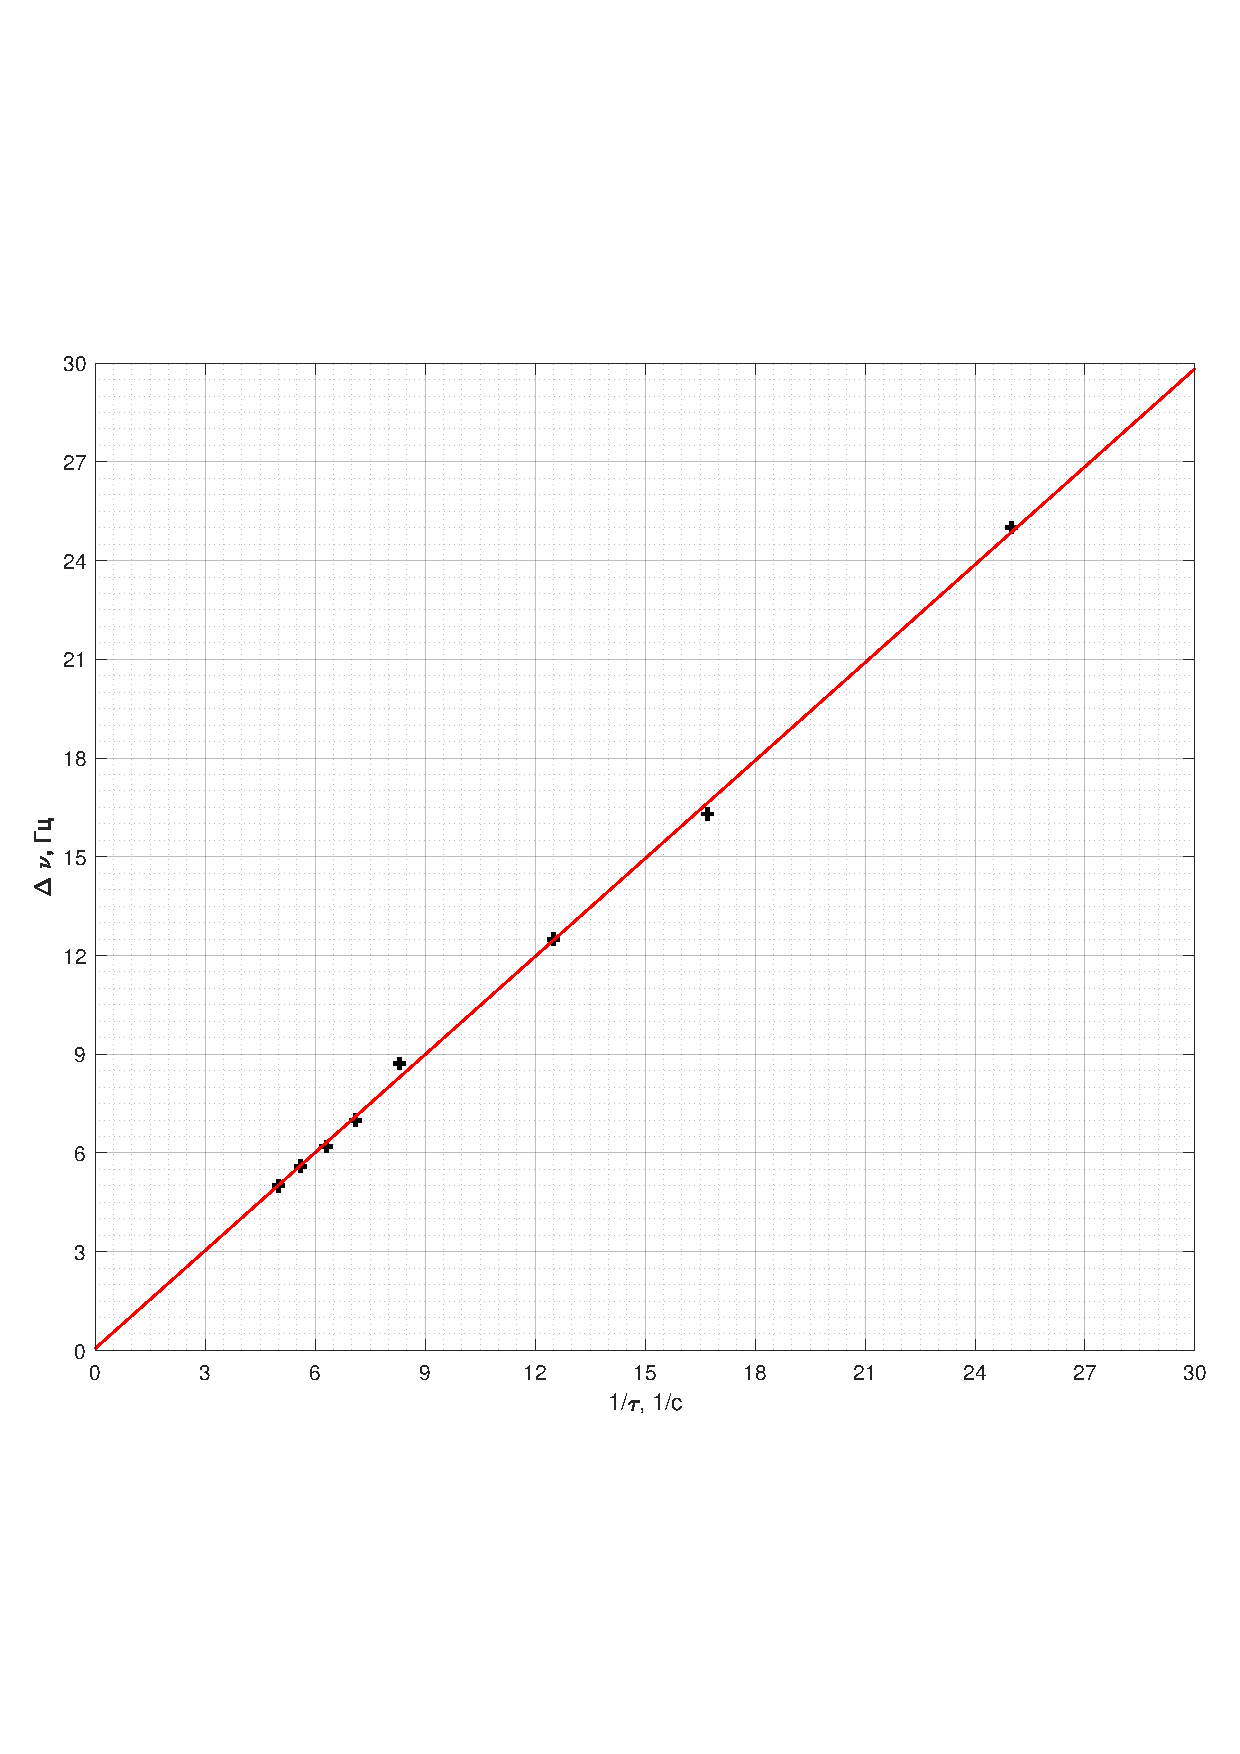
\includegraphics[width=\linewidth]{gr1.pdf}
	\caption{график зависимости $T_{\text{эксп}}$ от $T_{\text{теор}}$}
	\label{gr1}
\end{figure}
\end{center}

\subsection*{Критическое сопротивление и декремент затухания}

Теперь, считая $L = 200 $ мГн, вычислим  ёмкость. $\nu_0 = 5$ кГц $\Ra C = \dfrac{1}{(2\pi \nu_0)^2 L} = 5$ нФ. Тогда по формуле \eqref{Rkr}
$R_{\text{кр}} = 2 \sqrt{\dfrac{L}{C}} \approx$ 12.6 кОм.
Установим $C = 5$ нФ на магазине ёмкостей, будем наблюдать картину затухающих колебаний, изменяя $R$ от $0.1 R_{\text{кр}}$ до $ R_{\text{кр}} $. При этом сопротивление магазина, при котором колебания становятся апериодическими, примерно равняется $R_\text{эксп} =$ 6900 Ом $\approx 0.55 R_\text{кр}$.

Теперь, изменяя сопротивление от $0.1 R_\text{эксп} $ до $ 0.3 R_\text{эксп} $, будем измерять амплитуды колебаний, разделенных на $ n $ частей, для вычисления декремента по формуле \eqref{theta}. Погрешности амплитуд $  \sigma_{U_k} = \sigma_{U_{k+n}} = 0.1 $, таким образом 
$\sigma_{\Theta} = \Theta \sqrt{ \left( \dfrac{ \sigma_{U_k}}{U_k} \right)^2 + \left( \dfrac{ \sigma_{U_{k+n}} }{U_{k+n}} \right)^2 }$

\begin{table}[hbt!]
	\begin{center}
	\begin{tabular}{|c|c|c|c|c|c|c|c|c|c|c|}
		\hline
		$R$, $R_\text{кр}$ & $R$,Ом & $U_k$,дел & $U_{k+n}$,дел & $n$ & $\Theta$ & $\dfrac{1}{\Theta^2}$ & $R_\text{конт}$,Ом & $\dfrac{1}{R_\text{конт}^2}$, $10^{-6}$О$\text{м}^{-2}$ & $\sigma_{\theta}$ & $\sigma_{\frac{1}{\theta^2}}$ \\ \hline
		0.10     & 690   & 3.1       & 0.6         & 4 & 0.41     & 5.93                  & 711        & 1.98                                 & 0.07        & 2.01                             \\ \hline
		0.13     & 897   & 6.2       & 0.6         & 4 & 0.58     & 2.93                  & 918        & 1.19                                 & 0.10        & 0.98                             \\ \hline
		0.16     & 1104  & 5.0       & 0.6         & 3 & 0.71     & 2.00                  & 1125       & 0.79                                 & 0.12        & 0.67                             \\ \hline
		0.19     & 1311  & 3.8       & 0.7         & 2 & 0.85     & 1.40                  & 1332       & 0.56                                 & 0.12        & 0.41                             \\ \hline
		0.22     & 1518  & 6.8       & 0.9         & 2 & 1.01     & 0.98                  & 1539       & 0.42                                 & 0.11        & 0.22                             \\ \hline
		0.25     & 1725  & 6.4       & 0.6         & 2 & 1.18     & 0.71                  & 1746       & 0.33                                 & 0.20        & 0.24                             \\ \hline
		0.28     & 1932  & 6.2       & 0.4         & 2 & 1.37     & 0.53                  & 1953       & 0.26                                 & 0.34        & 0.27                             \\ \hline
		0.30     & 2070  & 6.2       & 1.5         & 1 & 1.42     & 0.50                  & 2091       & 0.23                                 & 0.10        & 0.07                             \\ \hline
	\end{tabular}
\caption{результаты измерений амплитуд}
\label{tab2}
\end{center}
\end{table}

По данным из таблицы \ref{tab2} построим график зависимости $\dfrac{1}{\Theta^2}$ от $\dfrac{1}{R_\text{конт}^2}$. См. рис. \ref{gr2}

\begin{center}
	\begin{figure}[hbt!]
		\centering
		\includegraphics[width=\linewidth]{gr2.pdf}
		\caption{график зависимости $\dfrac{1}{\Theta^2}$ от $\dfrac{1}{R_\text{конт}^2}$}
		\label{gr2}
	\end{figure}
\end{center}

Если заменить $\dfrac{1}{\Theta^2} = Y$, $\dfrac{1}{R_{\text{конт}}^2} = X$, то получаем, что $\dfrac{\Delta Y}{\Delta X} = 3.051 \cdot 10^6 \; \text{О}\text{м}^2$.
Тогда $R_\text{кр} = 2\pi \sqrt{\dfrac{\Delta Y}{\Delta X} } \approx 10.97$ кОм.
Погрешность равна $ \sigma_{R_\text{кр}} = R_\text{кр} \dfrac{1}{2} \dfrac{\sigma_a}{a} \approx 0.37$ кОм. 

Вычислим теоретическое значение $ R_\text{кр}  = 2\sqrt{\dfrac{L}{C}}$, где $ C = 5 $ нФ, $ L = 136 $ мГн. Получаем $ R_\text{кр} \approx 10.43 $ кОм, погрешность $ \sigma_{R_\text{кр}} = R_\text{кр} \dfrac{1}{2} \dfrac{\sigma_L}{L} \approx 0.29 $ кОм. 


\subsection*{Добротность}

По формуле \eqref{Q} посчитаем добротность через параметры контура $ C = 5 $ нФ, $ L = 136 $ мГн. Погрешность $ \sigma_Q = Q \dfrac{1}{2} \dfrac{\sigma_L}{L} $

Таким образом получаем:

\begin{center}
	$R = 2070$ Ом, \qquad $Q = 2.49 \pm 0.03$
	
	$R = 1725$ Ом, \qquad $Q = 2.99 \pm 0.04$
	
	$R = 897$ Ом, \qquad $Q = 5.75 \pm 0.07$
	
	$R = 690$ Ом, \qquad $Q = 7.48 \pm 0.09$
\end{center}

Теперь сделаем это по формуле $Q = \dfrac{\pi}{\Theta}$. Данные берём из таблицы \ref{tab2}. Погрешность равна $ \sigma_Q = Q \dfrac{\sigma_\Theta}{\Theta} $. 

\begin{center}
	$\Theta = 1.42$, \qquad $Q = 2.21 \pm 0.38$
	
	$\Theta = 1.18$, \qquad $Q = 2.66 \pm 0.45$
	
	$\Theta = 0.58$, \qquad $Q = 5.41 \pm 0.91$
	
	$\Theta = 0.41$, \qquad $Q = 7.66 \pm 1.11$
\end{center}


Теперь возьмём логарифмический декремент затухания, полученный через отношения радиусов спиралей, т.е. $ \Theta =  \dfrac{1}{n} \ln \dfrac{r_k}{r_{k+n}}$. Радиус мы будем измерять, наблюдая картину фазовых колебаний.

При $ R = 2070  $ Ом $ \ \ r_k = 0.6, \ \ r_{k+1} = 2.4 \ \Ra \ \Theta \approx 1.39$ 

При $ R = 1725  $ Ом $ \ \ r_k = 0.8, \ \ r_{k+1} = 2.6 \ \Ra \ \Theta \approx 1.18$ 

При $ R = 897  $ Ом $ \ \ r_k = 1.1, \ \ r_{k+2} = 3.4 \ \Ra \ \Theta \approx 0.56$ 

При $ R = 690  $ Ом $ \ \ r_k = 1.4, \ \ r_{k+2} = 3.6 \ \Ra \ \Theta \approx 0.47$ 

Погрешность считается аналогично формулам выше. Итого получаем для спирали:

\begin{center}
	$\Theta = 1.39$, \qquad $Q = 2.27 \pm 0.43$
	
	$\Theta = 1.18$, \qquad $Q = 2.66 \pm 0.56$
	
	$\Theta = 0.56$, \qquad $Q = 5.57 \pm 0.71$
	
	$\Theta = 0.47$, \qquad $Q = 6.65 \pm 0.88$
\end{center}


\section*{Выводы}
В этой работе мы изучили свободные колебания в электрическом контуре: сначала измеряли периоды при $ \gamma \approx 0 $, затем находили критическое сопротивление и изучали колебательный контур при сопротивлениях порядка (0.1 --- 0.3) $R_{\text{кр}}$. Мы исследовали зависимость логарифмического декремента затухания от сопротивления контура, а также добротности от параметров контура и от декремента.

\begin{table}[h!]
	\centering
	\caption{Расчет критического сопротивления}
	\begin{tabular}{|c|c|c|c|}
		\hline
		\multirow{2}{*}{$  L $} & \multicolumn{3}{|c|}{$ R_\text{кр} $} \\
		\cline{2-4}
		& Теор. & Подбор & Граф.  \\
		\hline
		$ 136 \pm  5 $ мГн   & $ (10.43 \pm 0.29) $ кОм & 12.6 кОм & 	$ (10.97 \pm 0.37) $ кОм \\
		\hline
	\end{tabular}
\end{table}

\begin{table}[h!]
	\centering
	\caption{Расчет добротности}
	\begin{tabular}{|c|c|c|c|}
		\hline
		\multirow{2}{*}{$ R $} & \multicolumn{3}{|c|}{$ Q $} \\
		\cline{2-4}
		& Теор. & $ f(\Theta) $ & Спираль \\
		\hline
		2070 Ом & $ 2.49 \pm 0.03 $ & $ 2.21 \pm 0.38 $ & $ 2.27 \pm 0.43 $ \\
		\hline
		1725 Ом  & $ 2.99 \pm 0.04 $ & $ 2.66 \pm 0.45 $  & $ 2.66 \pm 0.56 $ \\
		\hline
		897 Ом  & $ 5.75 \pm 0.07 $ & $ 5.41 \pm 0.91 $  & $ 5.57 \pm 0.71 $ \\
		\hline
		690 Ом  & $ 7.48 \pm 0.09 $ & $ 7.66 \pm 1.11 $  & $ 6.65 \pm 0.88 $ \\
		\hline
	\end{tabular}
\end{table}

Как можно видеть, полученные результаты совпадают в пределах погрешности. Значение критического сопротивления, полученное подбором, достаточно сильно отклонилось от двух других, потому что в нём мы брали примерное значение $L$.

\end{document}